\documentclass[12pt,letterpaper, onecolumn]{exam}
\usepackage{amsmath}
\usepackage{amssymb}
\usepackage{graphicx}
\usepackage{caption}
\graphicspath{ {./images/} }
\usepackage[lmargin=71pt, tmargin=1.2in]{geometry}
\lhead{Mustafa Rashid\\}
\rhead{Problem Set 1\\}
\chead{\hline} 
\thispagestyle{empty} 
\newcommand*{\setdef}[1]{\left\{#1 \right\}} 

\begin{document}
	
	\begingroup  
	\centering
	\LARGE Multi-variable Calculus\\
	\LARGE Problem Set 1\\[0.5em]
	\large \today\\[0.5em]
	\large Mustafa Rashid\par
	\large Fall 2024\par
	\endgroup
	\rule{\textwidth}{0.4pt}
	\pointsdroppedatright
	\printanswers
	\renewcommand{\solutiontitle}{\noindent\textbf{Ans:}\enspace}  
	
	
	% EXERCISE SET 1.1
	\begin{questions}
		
		\question What is wrong with each of the following statements? Explain briefly.
		\begin{parts}
			\part "In 3-space $y=1$ is a line parallel to the x-axis."
			\part "The graph of the function $f(x,y) = x^2 + y^2$ is a c
		\end{parts}
		\begin{solution}
			A1.
			
			\begin{parts}
				\part In 2-space $y=1$ is a line parallel to the $x$-axis, however in 3-space $y=1$ is not a line but a plane that is parallel to the $x$-axis.
				\part For the function $f(x,y)=x^2+y^2$ to be a circle it has to be a single variable function with value of $x$ or $y$ or $z$ set to a constant c. This will then be a graph in 2-space of a circle centered at $(0,0)$ with radius $\sqrt c$. However, the multi-variable function $f(x,y)=x^2+y^2$ is not a circle but it is bowl shaped with contour diagrams showing circles, with radii that vary as $f(x,y)$ is set to different constants $c$ where $c\geq 0$, concentric at $(0,0)$
			\end{parts}
		\end{solution}
		
		\pagebreak
		\question Sketch a graph of the surface $x^2+y^2+z^2 =9$ and briefly describe it in words, geometrically. Make sure you mark the coordinates of at least one point in your sketch to reflect the scale of the sketch.
		\begin{solution}
			A2.
			\\
			\\
			\\
			\\
			\\
			\\
			\\
			\\
			\\
			\\
			\\
			\\
			\\
			\\
		\end{solution}
	
		\question The following problems concern the concentration, $C$, in mg/liter, of a drug in the blood as a function of $x$, the amount, in mg, of the drug given and $t$, the time in hours since the injection. For $1\leq x \leq 4$ and $t \geq 0$ we have $C = f(x,t) = te^{-t(5-x)}$.
		\begin{parts}
			\part Find $f(3,2)$. Give units and interpret in terms of drug concentration.
			\part Graph the single variable function $f(4,t)$ (in the variable $t$) and explain its significance in terms of drug concentration.
			\part Graph $f(a,t)$ for $a=1,2,3,4$ on the same axes. Describe how the graph changes as $a$ increases and explain what this means in terms of drug concentration. 
		\end{parts}
		\begin{solution}
			A3.
			\begin{parts}
				\part $C = f(x,t) = te^{-t(5-x)}$\\
				$f(3,2) = ?$\\
				$x=3$ meaning that 3 mg of the drug was given\\
				$t=2$ meaning that 2 hours have passed since the injection\\
				$C$ or concentration of drug in mg/liter of 3 mg after 2 hours will be:\\
				$C = 2e^{-2(5-3)} = 0.04$ mg/liter
				
				The concentration in blood of 3 mg of the drug after 2 hours is 0.04 mg/liter 
				
				\part Drug concentration (mg/l) as a function of $x$, the amount in mg of the drug given, and $t$, the time in hours since the injection with $x$ held constant at 4 mg\\
				\makebox[0pt][l]{
					\begin{minipage}{\textwidth}
						\centering
						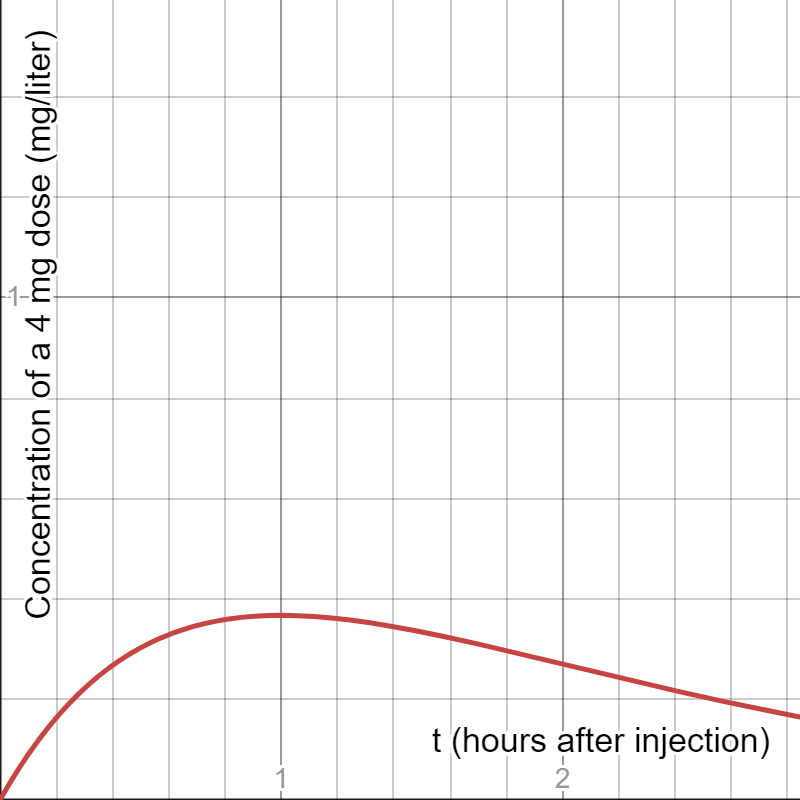
\includegraphics[width=.4\textwidth]{question3b}
						\captionof{figure}{}
					\end{minipage}
				}
				
				
				\part As more mg of the drug is given, the maximum concentration of the dose in the blood in mg/l increases. This can be seen on the graphs as the peaks of the functions $f(4,t)$, $f(3,t)$, $f(2,t)$, and $f(1,t)$. The highest peak is at $a=4$ and the lowest peak is at $a=1$. The time $t$ hours since the injection for the drug to reach its maximum concentration increases as the value of $a$ or the the value of the dose given increases.\\
				\makebox[0pt][l]{
					\begin{minipage}{\textwidth}
						\centering
						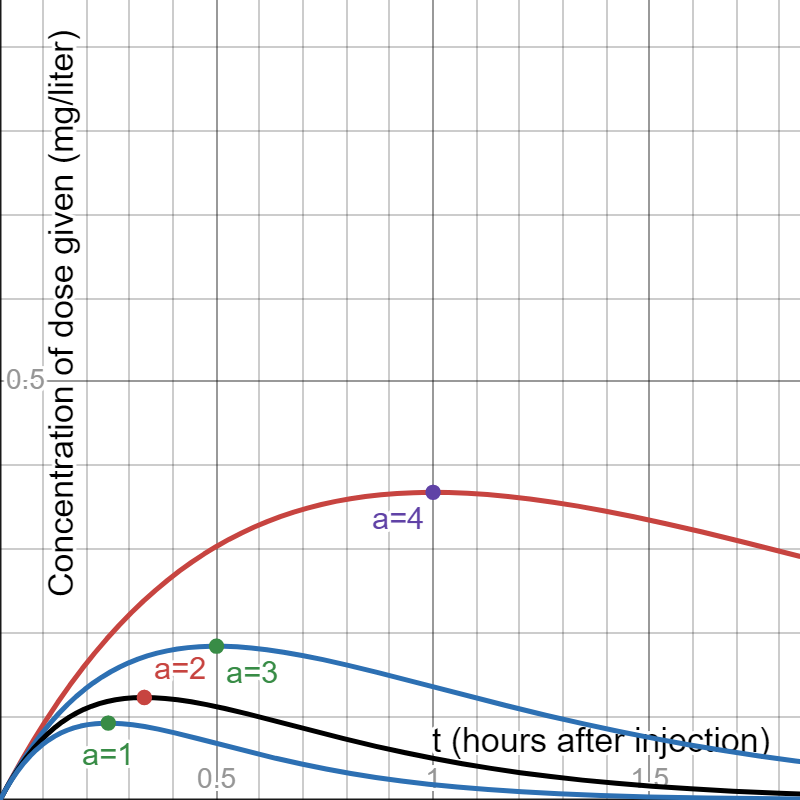
\includegraphics[width=.4\textwidth]{question3c}
						\captionof{figure}{}
					\end{minipage}
				}
				
				\medskip
				

			\end{parts}
		\end{solution}
		
		\question Without a calculation or computer, match the functions (a)-(f) with their cross-sections with $x$ fixed in the Figure 3. Explain your reasoning
			
			\makebox[0pt][l]{%
				\begin{minipage}{\textwidth}
					\centering
					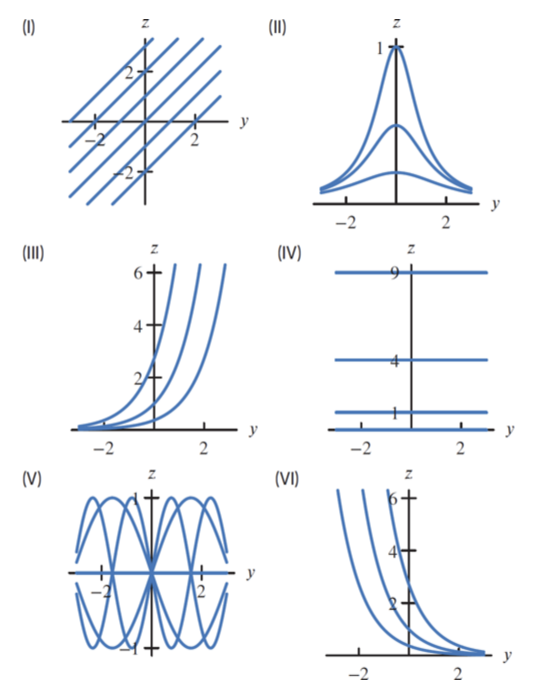
\includegraphics[width=.4\textwidth]{question4}
					\captionof{figure}{}
					\label{fig:fig1}
				\end{minipage}
			}
			
			\medskip
			\begin{solution}
			A4.
			\begin{parts}
				\part 
				\\
				\\
				\part
				\\
				\\
				\part
				\\
				\\
				\part
				\\
				\\
				\part
				\\
				\\
				\part
			\end{parts}
		\end{solution}
	\end{questions}
\end{document}
